\chapter{Introduction}
\label{chapter:Introduction}



Here starts the thesis with an introduction. Please use nice latex and bibtex entries \cite{latex}. Do not spend time on formating your thesis, but on its content. 
 
\section{Motivation}
\itemize 
\item Object recognition by manipulation
\item Leverage on manipulation capabilities
\item Perception in Clutter

\label{sec:intro}
A service robot operating in human environments may be
required to perform complex  dexterous manipulation tasks in a variety
of  conditions.  For example, when setting a table~\cite{iros10kcopman} the robot is likely to be
confronted with a cluttered unstructured scene\footnote{Following the discussion at the Clutter12
workshop at RSS 2012 we acknowledge that this is a ``laboratory clutter'' where the degree of difficulty
is similar to the scenes from the related works but still inferior to the real world clutter.} like the example shown
in \ref{fig:tracking_dists}.  In order to successfully perform this task,
the robot must be able  to detect the individual objects.  Without the
ability  to interact  with the  environment,  it is  difficult  to
distinguish between the object boundaries and texture patterns, particularly in the presence of objects of similar colors, shapes and sizes. 

To demonstrate this we tested three state-of-the-art segmentation algorithms operating in depth, RGB and RGBD
space respectively on the given scene. The results are shown in \ref{fig:tracking_dists}. We notice that they are far
from being optimal in the cases of a) same color objects (a coffee mug and a saucer), 
b) similar shape objects and occlusions (a white and a blue box), c) stacked objects (an egg and a plate)
and also in the case of d) a sensor
default (cutlery in this case appears transparent to the Kinect sensor). Following structure from motion
approaches, one could observe the scene from various views and apply merging of hypotheses.
This approach would however fail in the case of non-navigable spaces for the robot.
While one can certainly fine tune the algorithms' parameters for a certain setup and 
environment, it is easier and arguably more natural to exploit the robot's embodiment
and interaction capabilities in order to obtain a better understanding of its environment.
Reaching out to get a sense of what is around is the way how infants get to know their
``near space'' according to Piaget's theory of spatial cognition in the sensorimotor stage 
(until the age of 2), and getting a hold of connectivity (i.e. object unity) is an important
factor in the infant's understanding of objects at that stage \cite{infants}.

\setlength{\tabcolsep}{0.1em}
\begin{figure}[ht]
%\centering
\begin{tabular}{cccc}
\multicolumn{2}{c}{\multirow{-6}{*}{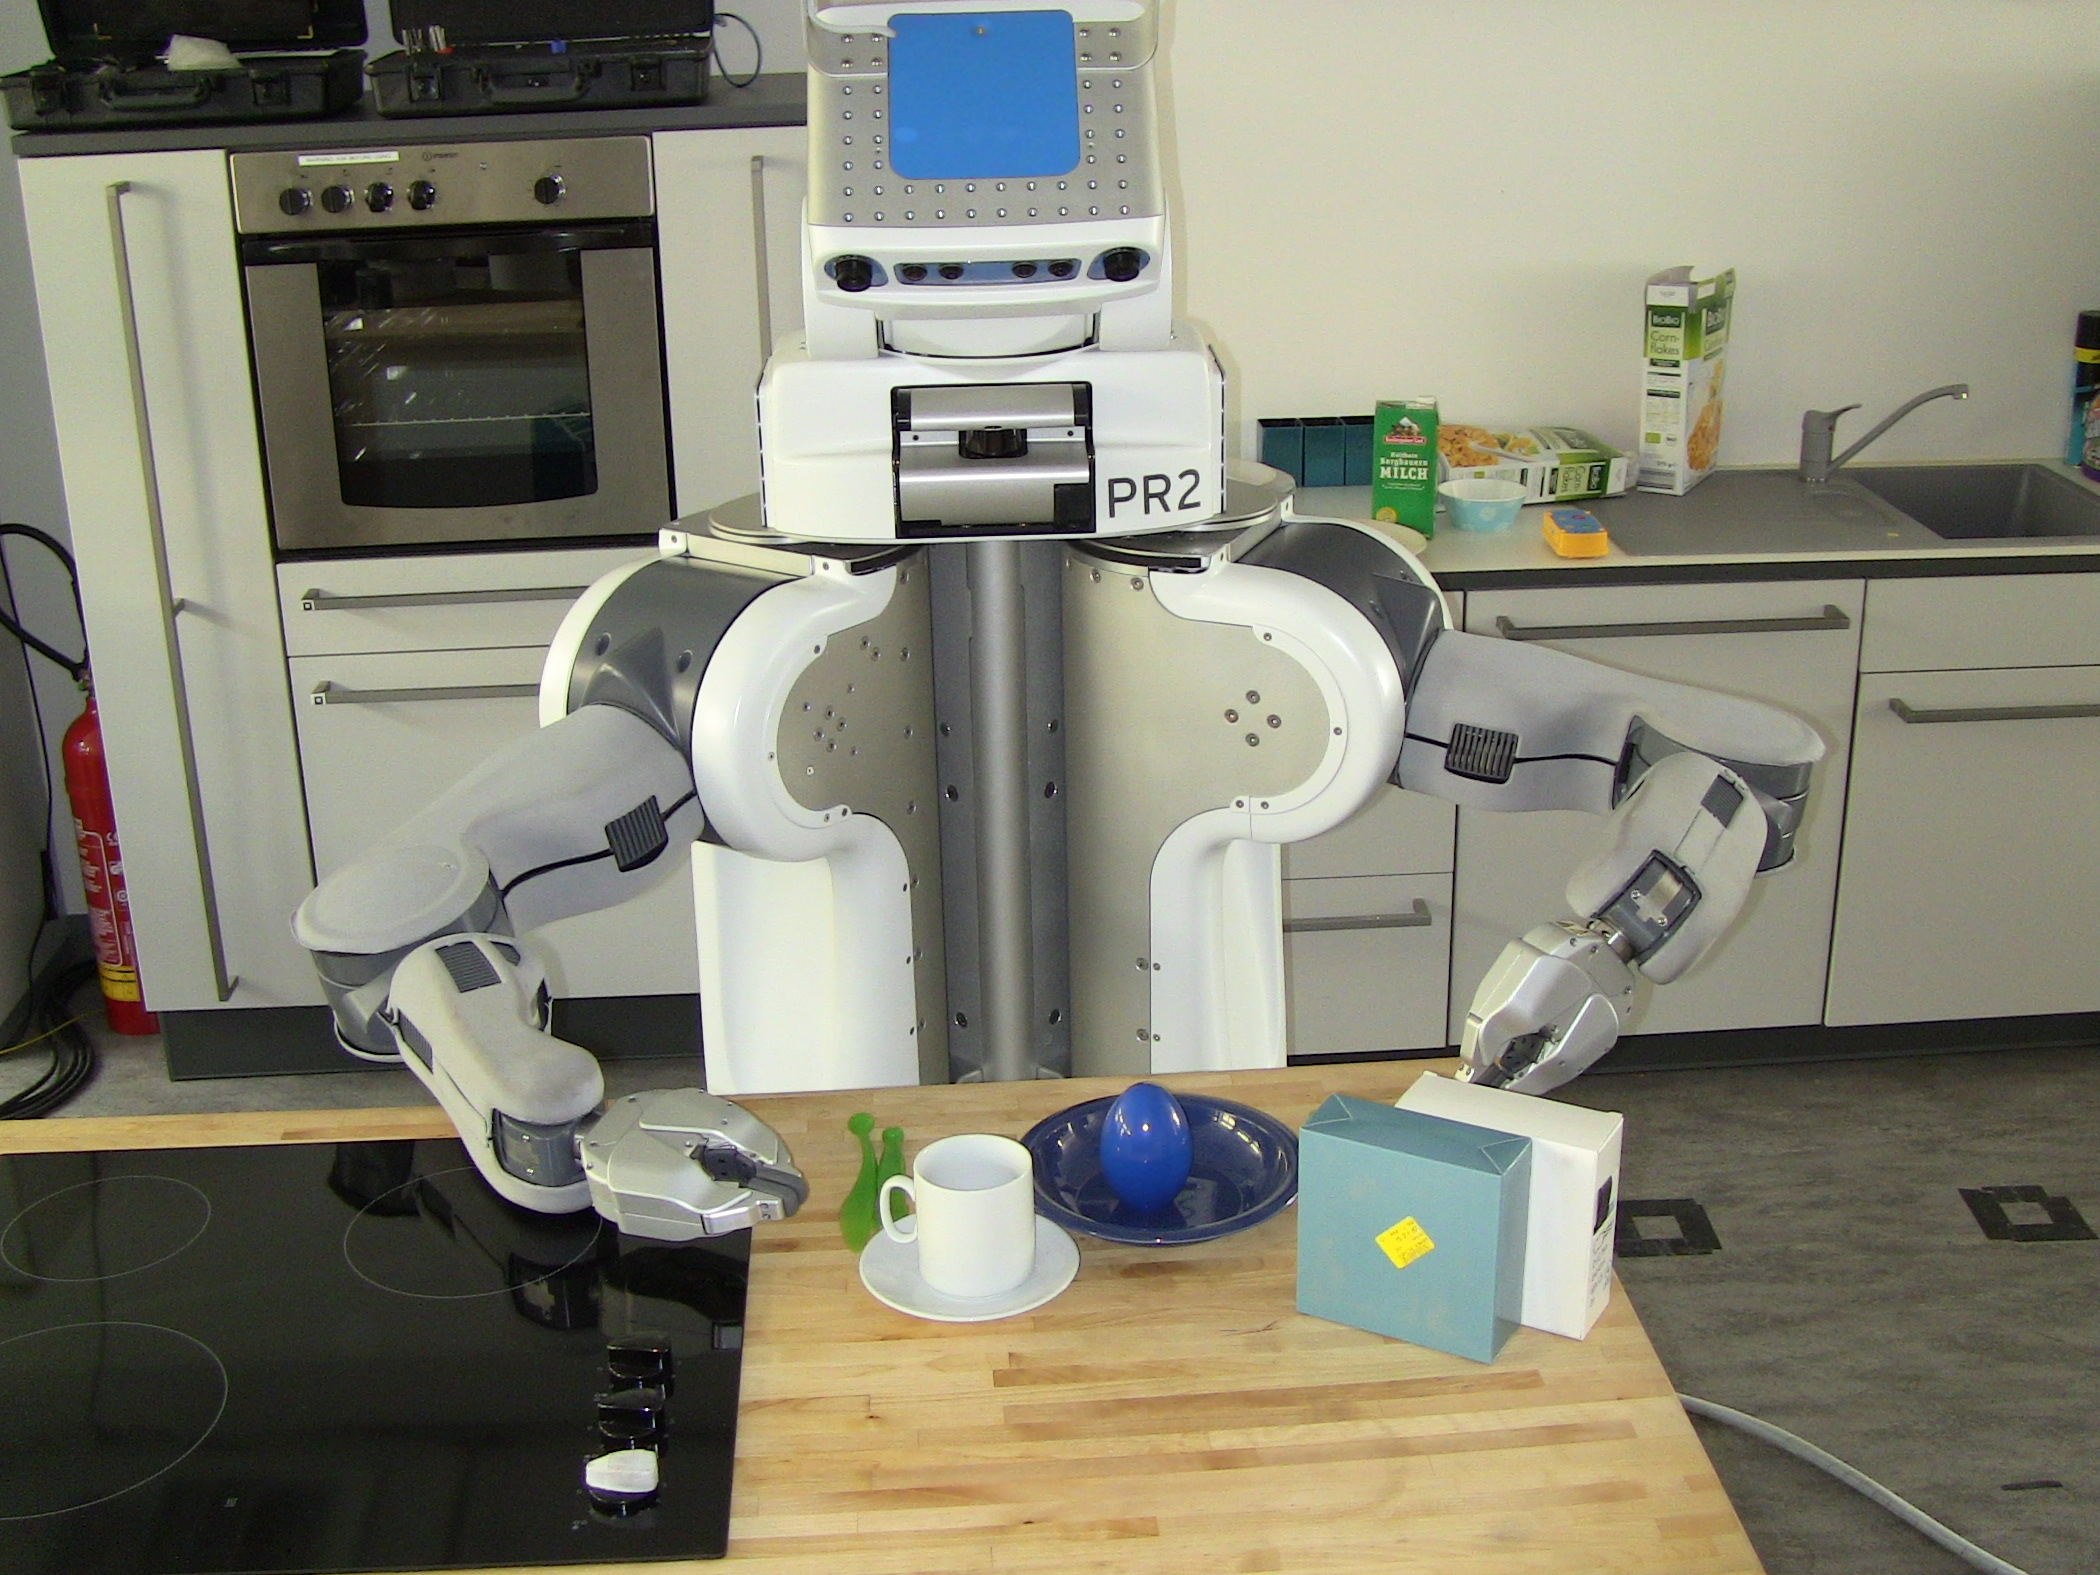
\includegraphics[width=0.5\columnwidth]{figures/teaser/IMG_0395.JPG}
}} & 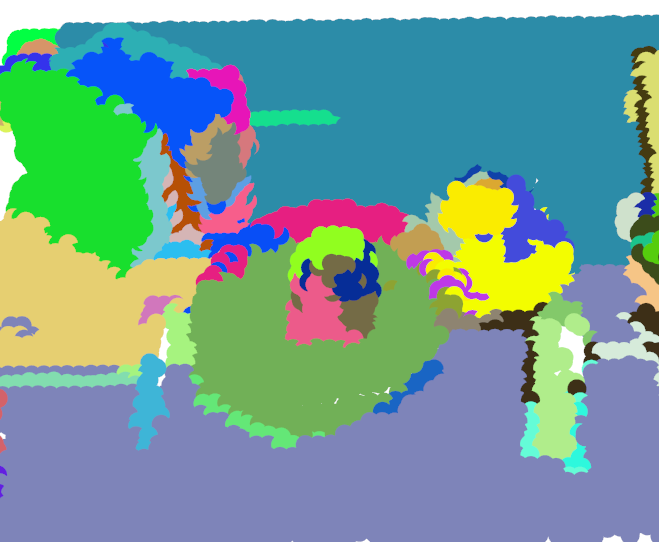
\includegraphics[width=0.23\columnwidth]{figures/segmentation_others/region_growing_rgb.png} 
&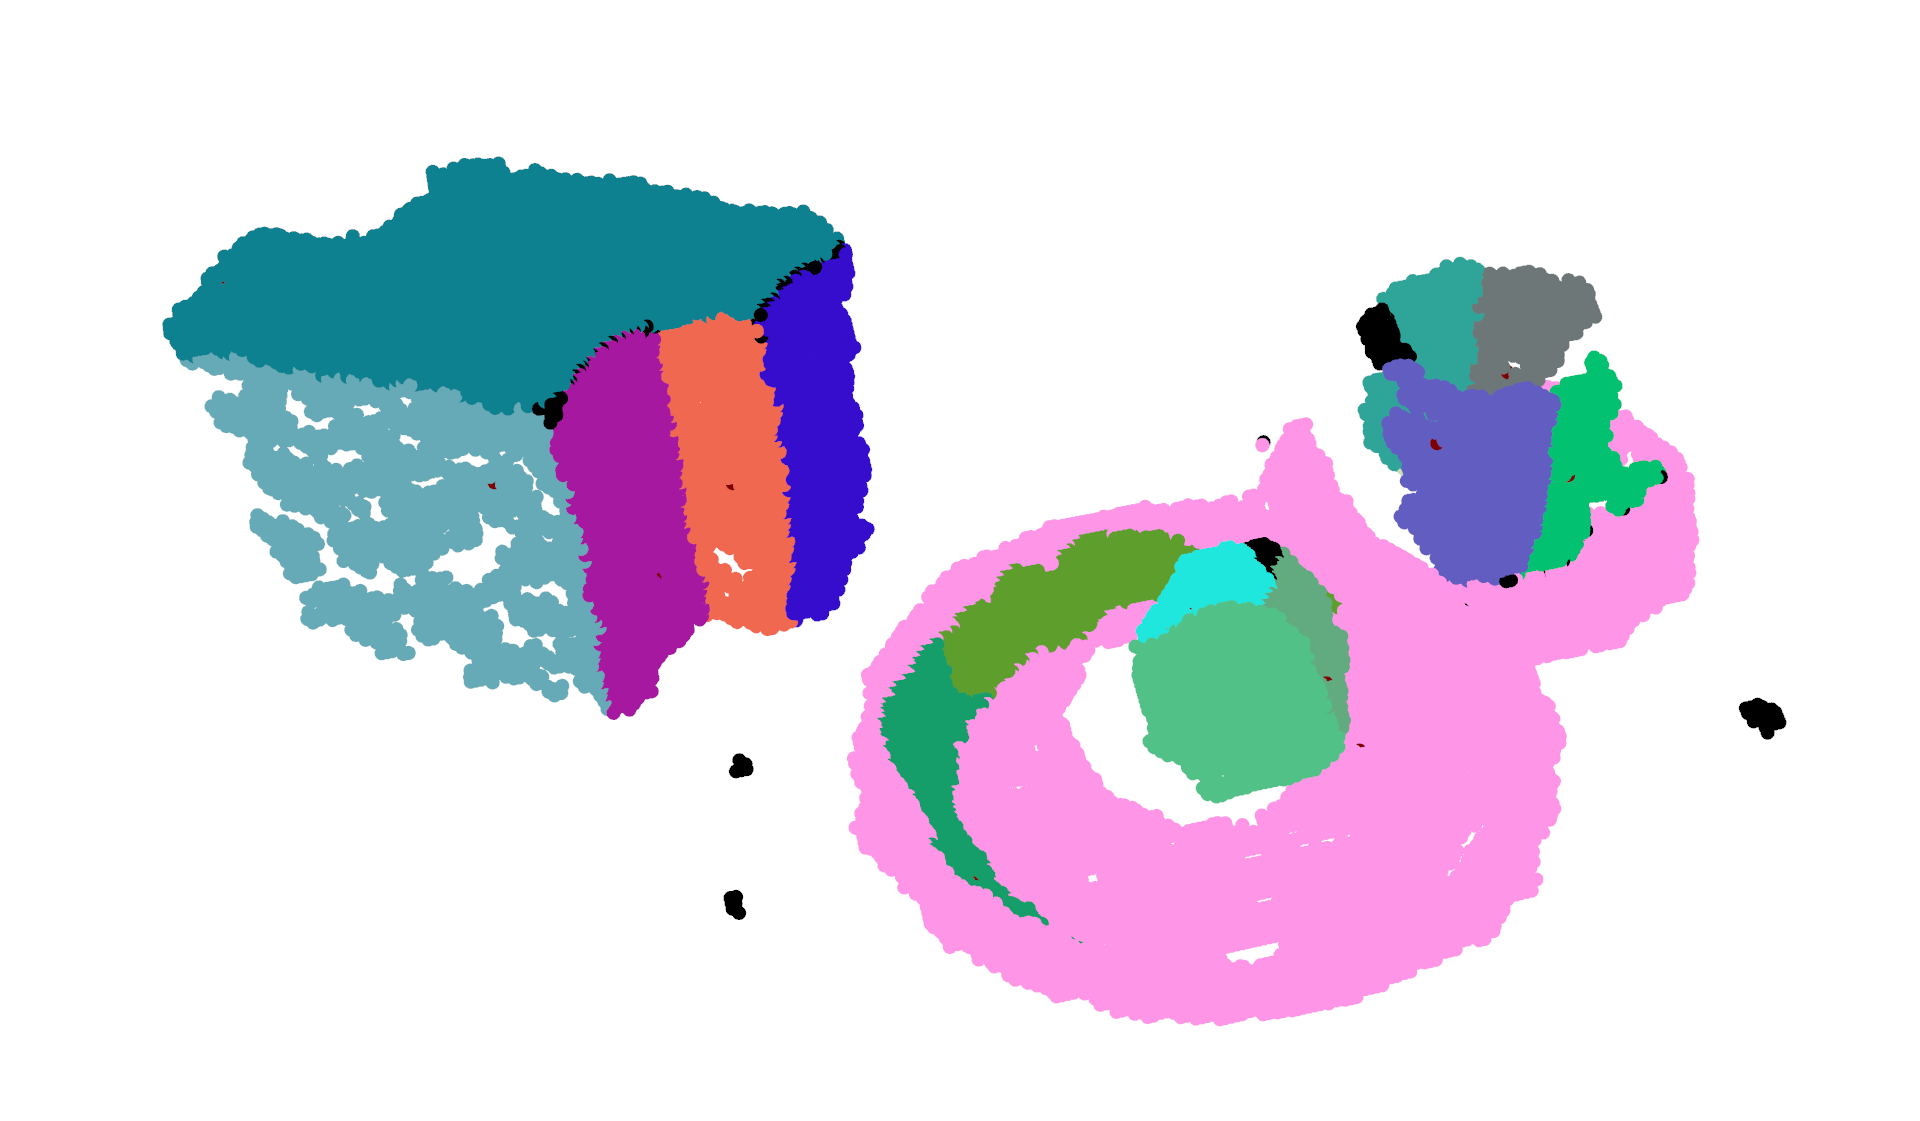
\includegraphics[width=0.23\columnwidth]{figures/segmentation_others/part-graph-hashing.png} \\
\multicolumn{2}{c}{} & \includegraphics[width=0.23\columnwidth]{figures/segmentation_others/graph-based.png} 
&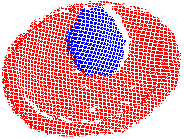
\includegraphics[width=0.23\columnwidth]{pictures/teaser_egg_result-cropped.png} \\
%\multicolumn{2}{c}{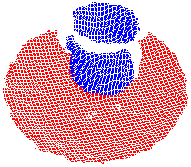
\includegraphics[width=0.38\columnwidth]{pictures/113-cropped.png}} 
\multicolumn{2}{c}{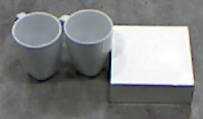
\includegraphics[width=0.45\columnwidth]{figures/3objects/after_push.jpg}}
& \multicolumn{2}{c}{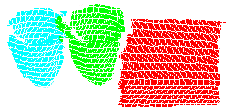
\includegraphics[width=0.45\columnwidth]{figures/3objects/segmented.png}}
\end{tabular}
\caption{Top-left: The service robot PR2 aiming to segment the scene
  consisting of textureless object. Results  of  the   scene segmentation
  using Region  Growing  method~\cite{RGBRegionGrowing} (top-right, NW), Part-Graph-based 
  Hashing~\cite{marton12SC} method (top-right, NE) and Graph-based  
  segmentation method~\cite{Felzenszwalb}   (top-right, SW). These methods work in depth, RGB and RGBD 
  space respectively and all underachieve due to the complexity of this challenging task. 
  On the other hand blue egg on the blue plate was correctly segmented using the interactive approach presented in this paper (top-right, SE)
  Bottom row: 3 white objects segmented correctly showing the generality of the apporach for multiple objects.}
\label{fig:tracking_dists}
\end{figure}

\textbf{Our approach:} In this work we focus on proposing a solution for the cases a), b) and c) from above.
Similar  to Katz  et al.~\cite{Katz-WS-MM-ICRA2011}, Bergstrom et
al.~\cite{bergstrom11icvs}, and our earlier
work~\cite{bersch12interactive} we propose a system that uses
induced motions  in a scene to enable effective
object  segmentation.   Our  system   employs  a  combination  of  the
following  complementary techniques: pre-segmentation of a raw point cloud of a given scene from a single camera
view using part-graph-based hashing~\cite{marton12SC}, estimation
of a contact  point and a push direction of the robot's end effector~\cite{bersch12interactive}, RGBD feature
extraction and tracking using particle filtering-based tracking, graph-based feature trajectory 
clustering algorithm, and dense model reconstruction based on region growing in normal space.
There are three important assumptions in our system. First, that each item is a rigid  body and not subject
to large deformations when  interacting with  the robot's  end  effector or
other objects. We also assume that the objects are either flat (box-like) or round (cylinder-like),
which holds for most household objects in publicly available databases~\cite{marton11ijrr}, and
that in the tracking step the features do not get more than $50\%$ obstructed.

The evaluation was performed on 17 scenes with challenging arrangement of flat and
round objects of similar colors, shapes and sizes. $82\%$ of objects
were segmented correctly in these scenes.  Our system   is
available  as open source\footnote{\url{http://www.ros.org/wiki/interactive_segmentation_textureless}}
and can  be deployed  on a  robot equipped with either a 2D-camera and a depth
camera or Kinect camera and at least one arm.

Overall, we present the following main contributions for the
segmentation of scenes consisting of textureless tabletop
objects:
\begin{itemize}
\item A set of RGBD features suitable for the tracking of
  flat and round textureless object REF%(\secref{3dfeatures});
%\item A particle filtering-based tracking algorithm for above features;
\item A graph-based algorithm  for the clustering of 3D-feature
trajectories, in which graph edges measure the dissimilarities between the RGBD
features' distances REF%(\secref{clustering});
\item The inclusion of a static scene pre-segmentation algorithm
  and a probabilistic method for the detection of over or under-segmentation REF%(\secref{static-seg});
\item A dense model reconstruction algorithm that makes use of the already clustered features REF%(\secref{dense_model});
\item And the integration of all the above into a pipeline using the
  Robot Operating System (ROS\footnote{\url{www.ros.org}}) as depicted in REF%\figref{pipeline}.
\end{itemize}



\section{Problem definition and goals}
\item Segmentation in clutter
\item Recognition in clutter

\section{Approach}
\item More details
\item General approach on clustering and so on	 


